\documentclass[tikz,border=10pt]{standalone}
\usepackage{tikz}
\usetikzlibrary{
    positioning,
    shapes.geometric,
    arrows.meta,
    calc,
    fit,
    backgrounds,
    matrix
}

\definecolor{hlca}{RGB}{70, 130, 180}
\definecolor{luca}{RGB}{205, 92, 92}
\definecolor{niche}{RGB}{60, 179, 113}
\definecolor{receiver}{RGB}{255, 165, 0}
\definecolor{attn}{RGB}{255, 215, 0}

\begin{document}
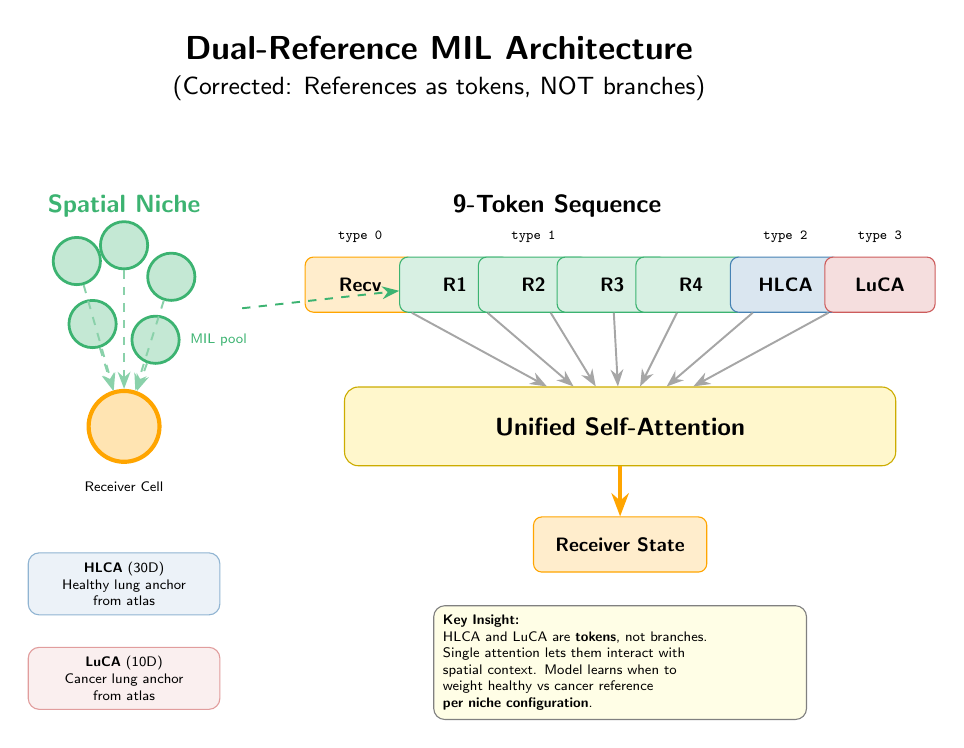
\begin{tikzpicture}[
    cell/.style={circle, draw=#1, fill=#1!30, minimum size=0.6cm, line width=1pt},
    token/.style={rectangle, draw=#1, fill=#1!20, rounded corners=3pt,
                  minimum width=1.4cm, minimum height=0.7cm, font=\scriptsize\sffamily\bfseries},
    arrow/.style={->, >=Stealth, line width=0.7pt, #1}
]

% Title
\node[font=\large\sffamily\bfseries] at (0, 4.5) {Dual-Reference MIL Architecture};
\node[font=\small\sffamily] at (0, 4) {(Corrected: References as tokens, NOT branches)};

% ============================================
% NICHE (bag of sender cells)
% ============================================
\node[font=\small\sffamily\bfseries, niche] at (-4, 2.5) {Spatial Niche};

% Sender cells in niche (multiple rings suggested)
\foreach \i/\x/\y in {1/-4.6/1.8, 2/-4.0/2.0, 3/-3.4/1.6, 4/-4.4/1.0, 5/-3.6/0.8} {
    \node[cell=niche] (s\i) at (\x, \y) {};
}

% Receiver cell (center of attention)
\node[cell=receiver, minimum size=0.9cm, line width=1.5pt] (recv) at (-4, -0.3) {};
\node[font=\tiny\sffamily, below=0.1cm of recv] {Receiver Cell};

% Dashed lines from senders to receiver
\foreach \i in {1,2,3,4,5} {
    \draw[arrow=niche!60, dashed] (s\i) -- (recv);
}

% ============================================
% TOKEN SEQUENCE (the key insight!)
% ============================================
\node[font=\small\sffamily\bfseries] at (1.5, 2.5) {9-Token Sequence};

% Tokens arranged horizontally
\node[token=receiver] (t_recv) at (-1, 1.5) {Recv};
\node[token=niche] (t_r1) at (0.2, 1.5) {R1};
\node[token=niche] (t_r2) at (1.2, 1.5) {R2};
\node[token=niche] (t_r3) at (2.2, 1.5) {R3};
\node[token=niche] (t_r4) at (3.2, 1.5) {R4};
\node[token=hlca] (t_hlca) at (4.4, 1.5) {HLCA};
\node[token=luca] (t_luca) at (5.6, 1.5) {LuCA};

% Type indicators
\node[font=\tiny\ttfamily, above=0.05cm of t_recv] {type 0};
\node[font=\tiny\ttfamily, above=0.05cm of t_r2] {type 1};
\node[font=\tiny\ttfamily, above=0.05cm of t_hlca] {type 2};
\node[font=\tiny\ttfamily, above=0.05cm of t_luca] {type 3};

% ============================================
% SINGLE SELF-ATTENTION (NOT dual branches!)
% ============================================
\node[rectangle, draw=attn!80!black, fill=attn!20, rounded corners=5pt,
      minimum width=7cm, minimum height=1cm, font=\small\sffamily\bfseries] (sattn) at (2.3, -0.3)
      {Unified Self-Attention};

% Connect tokens to attention
\foreach \tok in {t_recv, t_r1, t_r2, t_r3, t_r4, t_hlca, t_luca} {
    \draw[arrow=gray!70] (\tok) -- (sattn);
}

% From niche to ring tokens (MIL aggregation)
\draw[arrow=niche, dashed] (-2.5, 1.2) -- (t_r1);
\node[font=\tiny\sffamily, niche] at (-2.8, 0.8) {MIL pool};

% ============================================
% OUTPUT
% ============================================
\node[token=receiver, minimum width=2.2cm] (output) at (2.3, -1.8) {Receiver State};
\draw[arrow=receiver, line width=1.2pt] (sattn) -- (output);

% ============================================
% KEY INSIGHT BOX
% ============================================
\node[rectangle, draw=black!50, fill=yellow!10, rounded corners,
      font=\tiny\sffamily, text width=4.5cm, align=left] at (2.3, -3.3) {
    \textbf{Key Insight:}\\
    HLCA and LuCA are \textbf{tokens}, not branches.\\
    Single attention lets them interact with\\
    spatial context. Model learns when to\\
    weight healthy vs cancer reference\\
    \textbf{per niche configuration}.
};

% ============================================
% REFERENCE EXPLANATION
% ============================================
\node[rectangle, draw=hlca!60, fill=hlca!10, rounded corners,
      font=\tiny\sffamily, text width=2.2cm, align=center] at (-4, -2.3) {
    \textbf{HLCA} (30D)\\
    Healthy lung anchor\\
    from atlas
};

\node[rectangle, draw=luca!60, fill=luca!10, rounded corners,
      font=\tiny\sffamily, text width=2.2cm, align=center] at (-4, -3.5) {
    \textbf{LuCA} (10D)\\
    Cancer lung anchor\\
    from atlas
};

\end{tikzpicture}
\end{document}
